\chapter{Condiciones de estabilidad}

El capítulo anterior motiva al actual para presentar los resultados de la dinámica que produce la matriz de incidencias $\Lambda$ (Ec. \ref{eqn:MatrizIncidencias}) al integrarse en el sistema de Lotka-Volterra generalizado (ec. \ref{eqn:LK}) y linearizarse produciendo entonces la Matriz de Interacciones (\ref{eqn:MartizInteracciones}). En este capítulo se presentarán los resultados que produce cada etapa del proceso, así como sus características. Nuestra meta es alcanzar los diagramas de transición y compararlos con los resultados de May en sus distintos escenarios; con ello se busca caracterizar estas transiciones y proponer algunos criterios para que se tengan lugar estas transiciones.\\
\\
Para ello se consideraron 3 diferentes simulaciones que comparten algunas similitudes; en concreto la única diferencia es el número de especies o nodos en la red/matriz de incidencias: las simulaciones se consideraron para 25, 50 y 100 especies/nodos, siendo el último caso donde se generó más información. Para poder explorar los resultados de dejaron fijos la mayor cantidad de parámetros para poder observar cambios significativos, de todos los parámetros que hay en la ec. \ref{eqn:LK} únicamente se variaba la forma de la matriz de incidencias $\Lambda$ y que a su vez esta matriz depende de una probabilidad de conectividad $p$ y una fuerza promedio de interacción $\sigma$. En todas las simulaciones la tasa de crecimiento se dejó fija en $r=2$ y la capacidad de carga en $K=5$ para toda especie del sistema. Se integró el sistema con RK4 para un intervalo de tiempo entre 0 y 50 con un paso de integración de $h=0.01$.\\
\\
Además de estos parámetros, siempre se inicializó cada simulación con la condición inicial $\vec{x}_0=\vec{1}$ (dependiendo de la dimensión del sistema) y se consideraron dos escenarios\footnote{solo aplicca para $N=100$}: Matrices de incidencias estructuralmente simétricas y puramente aleatorias, tal y como se visualizó al final del capítulo anterior. En el apéndice (\ref{ch:Ap}), el lector puede darse una idea de como se realizó el proceso de las simulaciones. En cada escenario se presentó cierta cantidad de ruido en las gráficas de estabilidad, por lo que el número de simulaciones fue establecido en función de la disminución de dicho ruido.

\section{Series de tiempo}
Anteriormente se comentaba que las interacciones de la matriz de incidencias $\Lambda$ están volteadas con respecto de la matriz de interacciones $\mathcal{I}$ (ver Definición \ref{def:MatrizInteracciones}), la cooperación en $\mathcal{I}$ se da para las interacciones (++) mientras que para $\Lambda$ se da para $(--)$. Esto es muy importante no perderlo de vista puesto que al tener $N\gg 1$ especies, es difícil poder monitorear el signo de todas las interacciones que intervienen. Si tuviéramos un sistema puramente de competencia, es decir para toda $\alpha_{ij}\in\Lambda$ mayor o igual que cero, entonces no hay forma de que ninguna de las poblaciones participantes sobrepasen la capacidad de carga establecida, tal y como se pudo esbozar en el Ejemplo \ref{eg:2x2}. Por lo tanto obtendríamos series de tiempo caóticas para cada una de las especies por debajo de $K=5$.
\begin{figure}[h!]
	\centering
	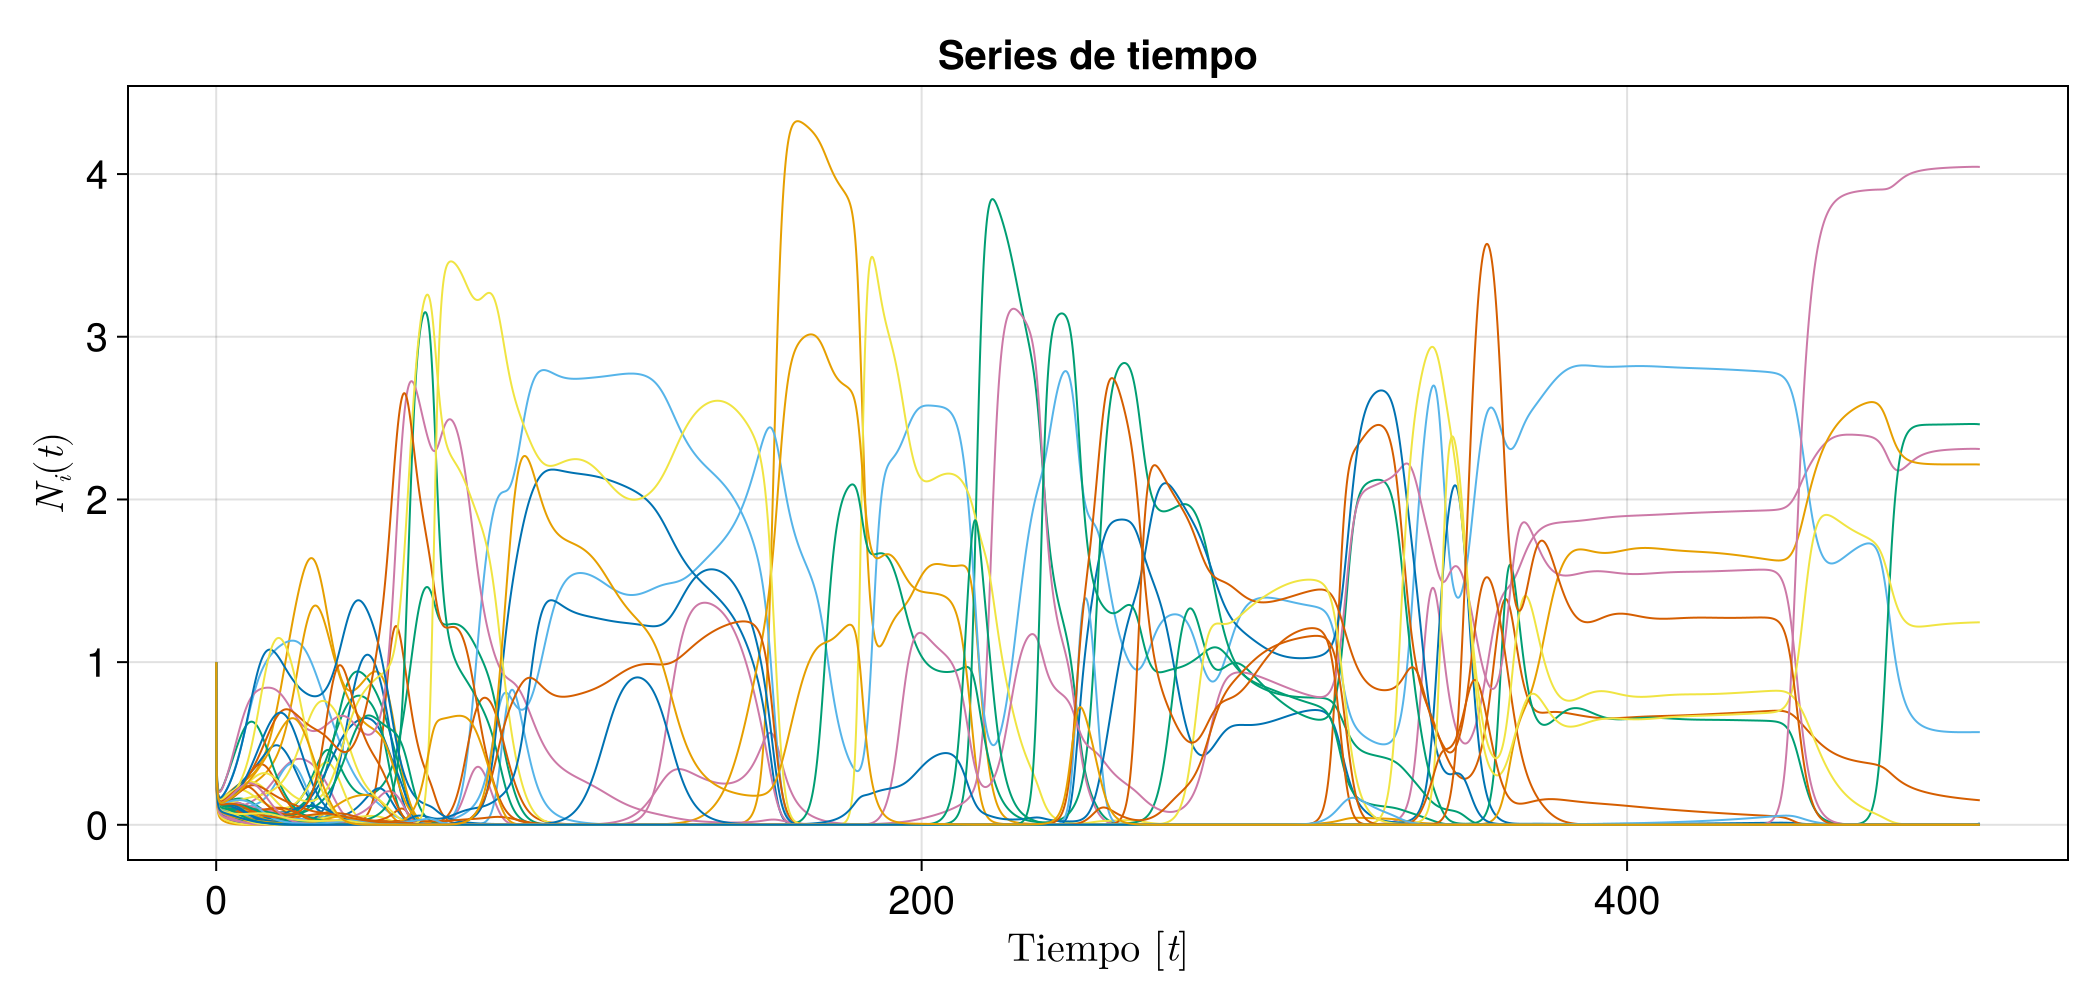
\includegraphics[scale=0.23]{../Imagenes/Seriesdetiempopositiva}
	\caption{Series de tiempo para el sistema de competencia de especies. Se emplea una matriz de incidencias de $100\times 100$ cuyas entradas son de una distribución uniforme en el intervalo [0,1]. En este caso particular no se considera a $\sigma$, solamente el tamaño de la red con $p=1.0$, es decir que es una red con el número máximo de enlaces posibles. En este caso la dinámica no sobrepasa la capacidad de carga puesto que las 100 especies se encuentran compitiendo y obedecen fielmente al comportamiento logístico.}
	\label{fig:Seriesdetiempopostiva}
\end{figure}

Una de las características que se encontró en esta clase de sistema en particular es que el tiempo en que tarda en estabilizarse es considerablemente mayor que en los sistemas donde consideraremos todas las interacciones antes mencionadas. Las poblaciones al estar confinadas por la capacidad de carga, tienen más oportunidad de interactuar entre sí pero esto genera que las constantes fluctuaciones prolonguen el tiempo de estabilización.
Por el contrario, el sistema generalizado sí excede la capacidad de carga lo que se traduce en una disminución de la cantidad de fluctuaciones que hace que el sistema pueda llegar al atractor en un tiempo mucho menor. Otro aspecto que se encontró en la red de competencias es que cuando es más conectada, tarda más tiempo en estabilizarse. Si generáramos una red de competencias con pocas conexiones ($p\leq 0.5$), el número de especies que compiten es considerablemente menor lo que produce que existan menor cantidad de fluctuaciones y a su vez las dinámicas de las poblaciones sean menos caóticas lo que hace que se pueda llegar a la estabilidad en un tiempo menor.\\
\\
En el Ejemplo \ref{eg:2x2CoopyDemás} del capítulo anterior, se observaba como las interacciones de cooperación $(--)$ en la matriz de incidencias $\Lambda$ genera la aparición de un atractor para ambas especies que se posiciona por arriba de la capacidad de carga (Figura (\ref{fig:CooperacionEspecies})). En el caso extendido a $N\gg 1$ especies ocurrirá lo mismo, solo que ahora tendremos un atractor $N$-dimensional. En este caso pueden haber especies que sobrepasen por mucho o poco la capacidad de carga, pero también cabe la posibilidad de que algunas no logren sobrepasarla y otras que lleguen a extinguirse. A continuación se muestran dos ejemplos diferentes
\begin{figure}[h!]
	\centering
	\includegraphics[scale=0.23]{../Imagenes/Series de Tiempo LK100}
	\caption{(\textbf{A}) Series de tiempo para el sistema de especies en competencia asociada a una matriz de incidencias de $100\times100$, con $\sigma=0.2$ y $p=0.35$. (\textbf{B}) Series de tiempo para el sistema de especies en competencia asociada a una matriz de incidencias de $100\times 100$ nodos con $\sigma=0.2$ y $p=0.5$}
	\label{fig:SeriesdeTiempoLK100}
\end{figure}

La diferencia evidente entre estas gráficas se da gracias a la matriz de incidencias, las interacciones que intervienen vienen de una fuerza de interacción promedio de $\sigma=0.2$ con diferentes probabilidades de conectividad, para $p=0.35$ y para $p=0.5$. El segundo caso corresponde con una red más conectada que el primero y eso se traduce al mismo tiempo en mayor oportunidad para crecer puesto que el crecimiento en este caso ronda hasta los 400 mientras que el otro escenario no pasa de 100. Esto podría interpretarse de la siguiente manera: entre más especies existan y cooperen entre sí, mayores serán sus crecimientos. Como se puede observar, el tiempo en que llegaron a estabilizarse fue menor a $t=50$, considerablemente menor a diferencia del caso de la Figura (\ref{fig:Seriesdetiempopostiva}). 

Sin embargo, el crecimiento no solamente depende de la cantidad de interacciones que existan (enlaces de la red), sino también de la fuerza de interacción promedio, entre mayor sea también se verá que la capacidad de crecimiento es proporcional a ello. Cuando se genera la matriz de incidencias en función de la matriz aleatoria (simétrica o no) y la matriz con entradas de una FDP normal centrada en $\mu=0$ se asume que existirán 50\% de valores positivos y 50\% de valores negativos distribuidos aleatoriamente en las 5 diferentes interacciones posibles\footnote{Si la matriz es puramente aleatoria son 5 posibles interacciones, sino entonces son 3.}. La presencia del comensalismo $(-0)$, depredación $(+-)$ o $(-+)$ y cooperación $(--)$ provoca numerosas especies logren superar la capacidad de carga del sistema para establecerse en el atractor $N$-dimensional, pero no hay que perder de vista que un ``exceso'' de estas interacciones genera inestabilidad y la posibilidad de que algunas de las especies divergan a infinito.
\\
\\
Los resultados de la Figura (\ref{fig:SeriesdeTiempoLK100}) en un principio se generaron a partir del tanteo y tomando como referencia la relación (\ref{eqn:parametroMay}), cabe preguntarse ¿cual debería se la cualidad de $\sigma$ y $p$ para que los sistemas de $N=100$ puedan hallar la estabilidad? La pregunta va encaminada a tratar de motivar la cualidad del parámetro crítico que relaciona $N$, $\sigma$ y $p$. Pero para llegar a ese punto primero se debe de conocer a la matriz de interacciones $\mathcal{I}$ resultante de realizar la integración del sistema y validar si lo que se nos muestra en estas gráficas de verdad es estabilidad (recordar la proposición \ref{prp:Atractores} acerca de la parte real de los eigenvalores de la matriz de interacciones).

\section{Matriz de interacciones}

En el capítulo anterior se definió el Jacobiano del sistema generalizado para poder determinar la matriz de interacciones, pero aún con ello no se ha presentado una forma de acceder a los puntos de equilibrio del sistema necesarios para dicho Jacobiano; debido a la naturaleza del sistema (considerando $N=100$), deben ser al menos 100 de ellos con diversas estabilidades. Calcularlos de manera analítica puede llegar a ser una tarea desafiante y poco redituable, pues de todos los puntos de equilibrio que puedan existir solo nos interesa el que es estable, y la mayoría de ellos podrían ser silla. La solución de ello por fortuna lo hallamos en el resultado de la integración numérica, como se puede ver en la Figura (\ref{fig:SeriesdeTiempoLK100}), al final de cada serie de tiempo se observa que las poblaciones llegan a estabilizarse. El último valor de cada población corresponde con una entrada del vector correspondiente al atractor que se encuentra contenido en el hiperespacio fase del sistema.\\
\\
Esto favorece a la construcción de los algoritmos que generan la matriz Jacobiana. Fácilmente se pueden programar las entradas de la matriz Jacobiana con base en la Definición \ref{def:MatrizInteracciones} y con ayuda de este vector correspondiente al atractor, se evalúa y finalmente se genera la matriz de interacciones $\mathcal{I}$ que tanto buscamos. Para tener certeza de la matriz de interacciones generada es importante validar que el sistema se estabiliza en un tiempo menor o igual (de preferencia menor) al tiempo final de la integración (en nuestro caso general para $t=50$). Se puede validar visualmente con las series de tiempo; una segunda validación sobre $\mathcal{I}$ es revisar que todos los elementos de su diagonal sean menores que cero, invocando así a la Proposición (\ref{prop:DiagonalI}. Se ha observado que cuando se ingresa un vector no correspondiente al punto de equilibrio estable, la diagonal de $\mathcal{I}$ contiene elementos positivos invalidando la proposición mencionada\footnote{Una hipótesis implícita de la Proposición \ref{prop:DiagonalI} es que para generar a $\mathcal{I}$ es necesario aplicar el Jacobiano de la Definición \ref{def:MatrizInteracciones} y evaluarlo en el atractor.}.
\\
\\
De esta forma podemos conocer las matrices de interacción de sistemas de competencia como los de la Figura \ref{fig:Seriesdetiempopostiva} y los sistemas generalizados de la Figura \ref{fig:SeriesdeTiempoLK100}. En este \href{https://github.com/rogve98/Tesis/tree/master/Notebooks/Datos/Ejemplo%20Jacobianos}{enlace}\footnote{Consultar: \url{https://github.com/rogve98/Tesis/tree/master/Notebooks/Datos/Ejemplo\%20Jacobianos}} el lector puede entrar a revisar por su cuenta el resultado de 4 matrices de interacción de sistemas que resultaron estables para los parámetros $N=100$, $\sigma=0.2$ y probabilidades $\{0.3,0.4,0.5,0.6\}$. Revisemos si en efecto estos ejemplos cumplen con la Poposición \ref{prop:DiagonalI}
\begin{tcolorbox}[colback=green!10!white, colframe=black, title=Entrada]
	\begin{minted}{julia}
using CSV, DataFrames
jacobianos = []
for i in 0.3:0.1:0.6
    ruta = "Datos/Ejemplo Jacobianos/Jacobiano100_p$i.s0.2.csv"
    df = CSV.read(ruta,DataFrame,header=false)
    push!(jacobianos,df)
end
jacobianos
	\end{minted}
\end{tcolorbox}

\begin{tcolorbox}[colback=red!10!white, colframe=black, title=Salida]
4-element Vector{Any}:\\
100×100 DataFrame
\end{tcolorbox}

Validando las diagonales de cada uno de las matrices de interacción consideradas se tiene

\begin{tcolorbox}[colback=green!10!white, colframe=black, title=Entrada]
	\begin{minted}{julia}
using LinearAlgebra
print(all(x -> x<0,diag(Matrix(jacobianos[1]))),", ")
print(all(x -> x<0,diag(Matrix(jacobianos[2]))),", ")
print(all(x -> x<0,diag(Matrix(jacobianos[3]))),", ")
print(all(x -> x<0,diag(Matrix(jacobianos[4]))))
	\end{minted}
\end{tcolorbox}

\begin{tcolorbox}[colback=red!10!white, colframe=black, title=Salida]
true, true, true, true
\end{tcolorbox}

El aspecto más importante de todas las matrices de interacción resultantes es que la diagonal no es homogénea como sí lo es en las matrices de May. Ocupando nuestro arreglo de Jacobianos veamos como son las disribuciones de los eigenvalores mediante la graficación de un histograma
\begin{figure}[h!]
	\centering
	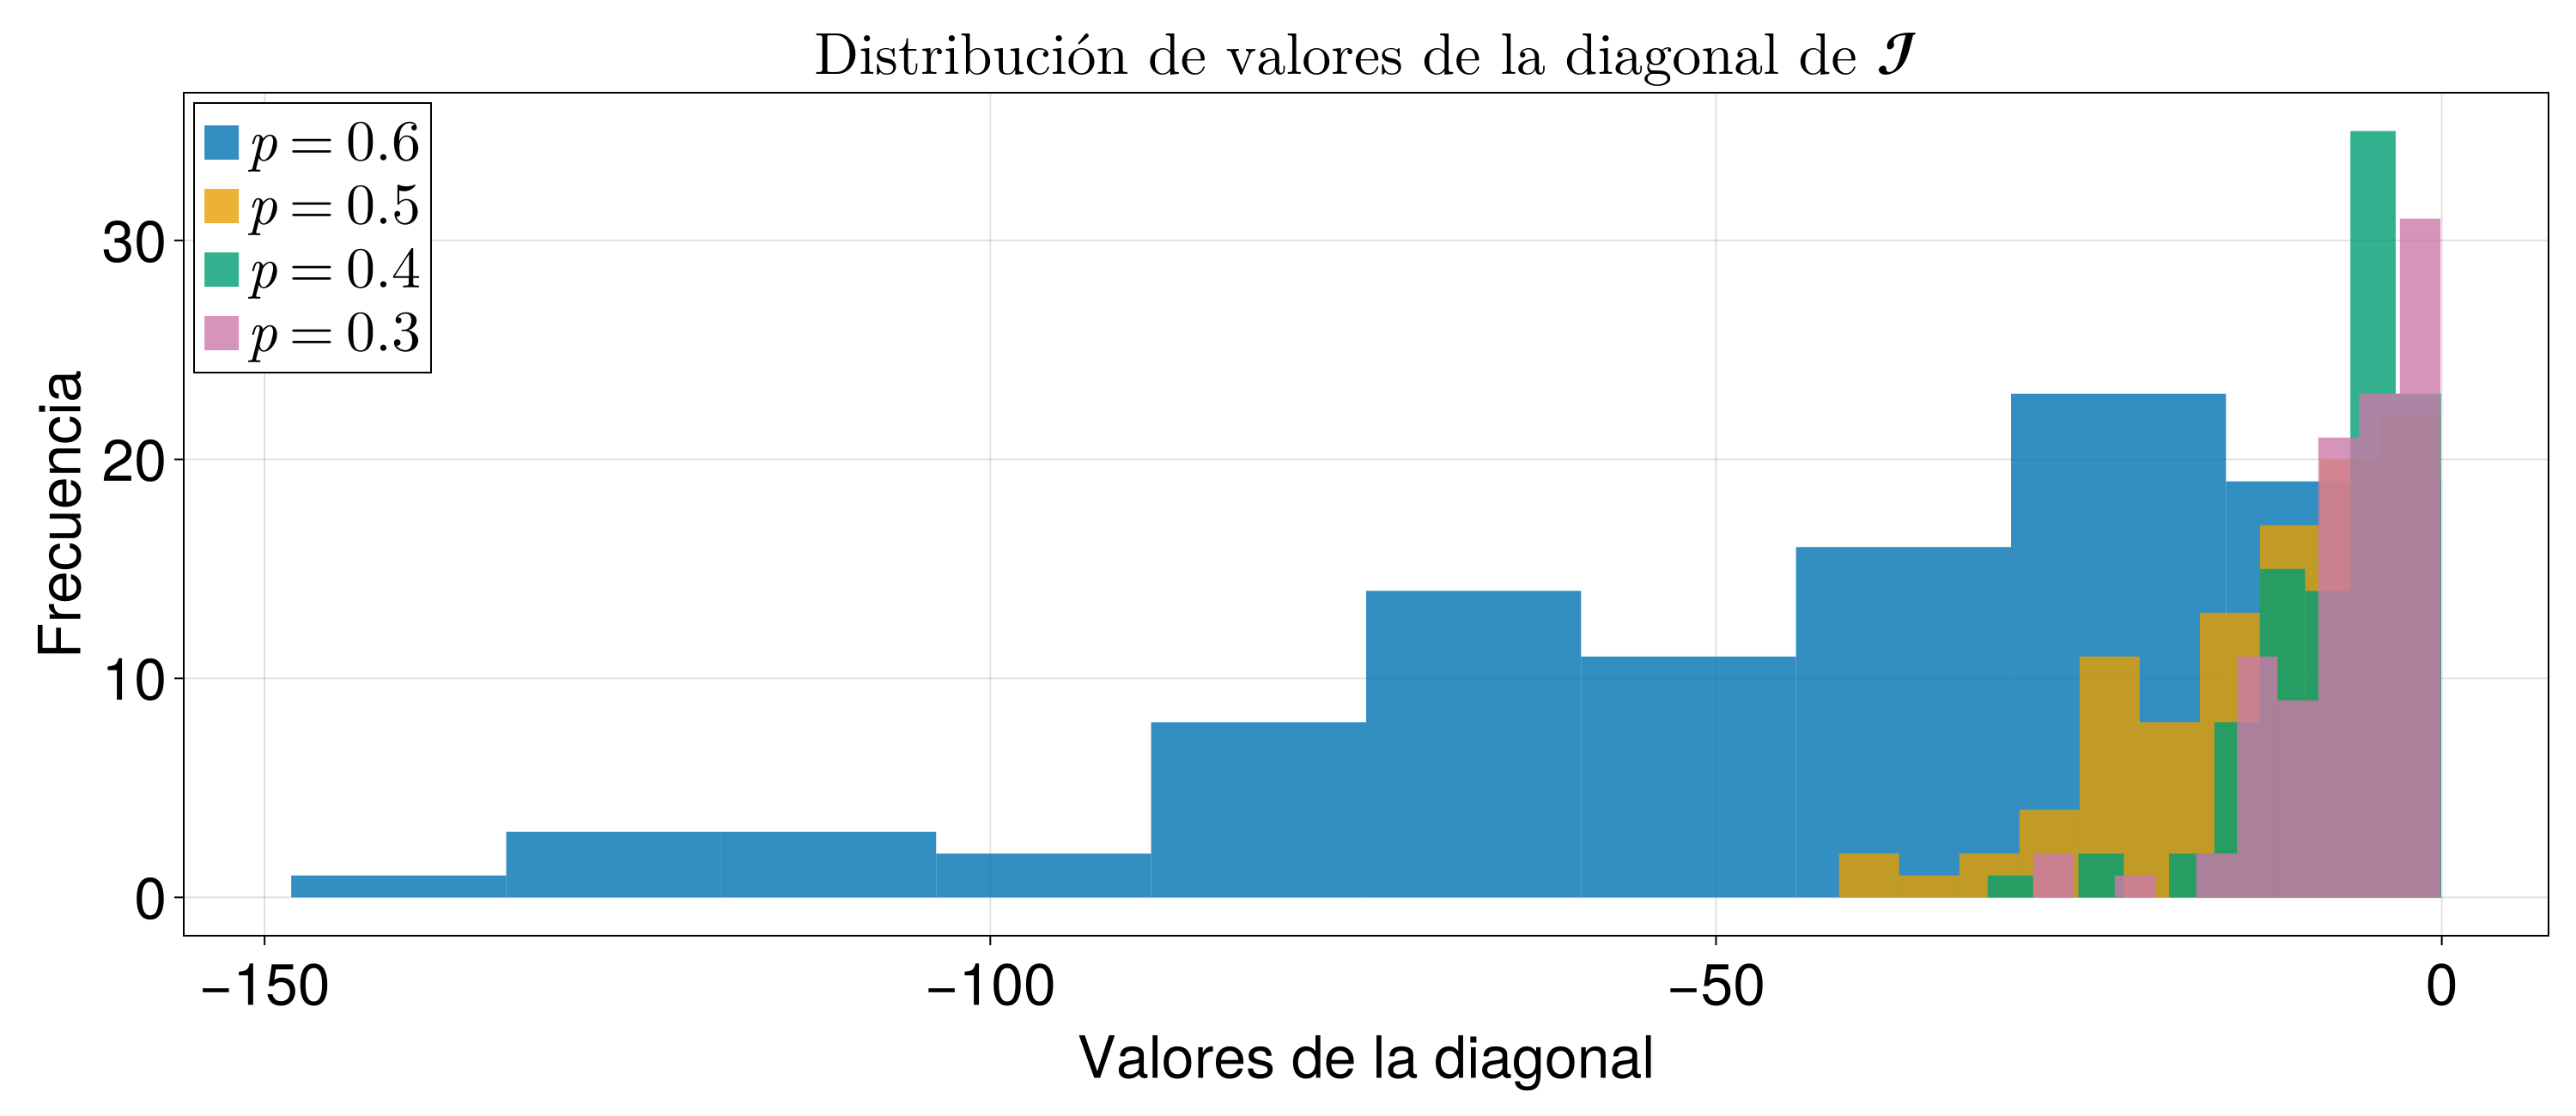
\includegraphics[scale=0.16]{../Imagenes/DistDiagonal}
	\caption{Distribución de la diagonal en matrices de interacción $\mathcal{I}$ del sistema generalizado para $N=100$, $\sigma=0.2$ y $p\in\{0.3,0.4,0.5,0.6\}$.}
	\label{fig:DistDiagonal}
\end{figure}

No solo no es homogénea sino que cuanto la probabilidad es mayor, la distribución es más dispersa hacia los valores negativos tal y como ocurre en el caso de $p=0.6$ en contraste con $p=0.3$. Este comportamiento es natural considerando el proceso de modelación e integración del sistema generalizado; suponer la diagonal homogénea es establecer un sistema demasiado ideal y por tanto difícilmente aproximable a la realidad. Esta propuesta pretende acercarse hacia la dinámica que presentan sistemas semejantes a la realidad, sin embargo aún sigue siendo muy teórico. 
\\
\\
En el capítulo pasado se vio que la importancia de la diagonal radica en la forma de la distribución de los eigenvalores del sistema en el plano complejo, englobado bajo la Ley Circular. En las matrices de May, la diagonal representaba el centro y radio del círculo que encerraba esta distribución de eigenvalores; a partir de esta distribución se puede visualizar de otra forma si el sistema es estable o no, viendo el signo de la parte real de los mismos. En nuestro caso, al no tener un radio/centro definido ¿qué podemos esperar de la distribución de eigenvalores de $\mathcal{I}$?
\newpage

\section{Leyes Circulares}

Viendo que la distribución de la diagonal no es homogénea en los sistemas generalizados, se debe analizar como es la distribución de lo eigenvalores en el plano complejo y si podría seguir la Ley Circular que establece May. Para ello se comenzará por revisar la distribución de eigenvalores de las matrices de interacción $\mathcal{I}$ que se invocaron en la sección anterior
\begin{figure}[h!]
	\centering
	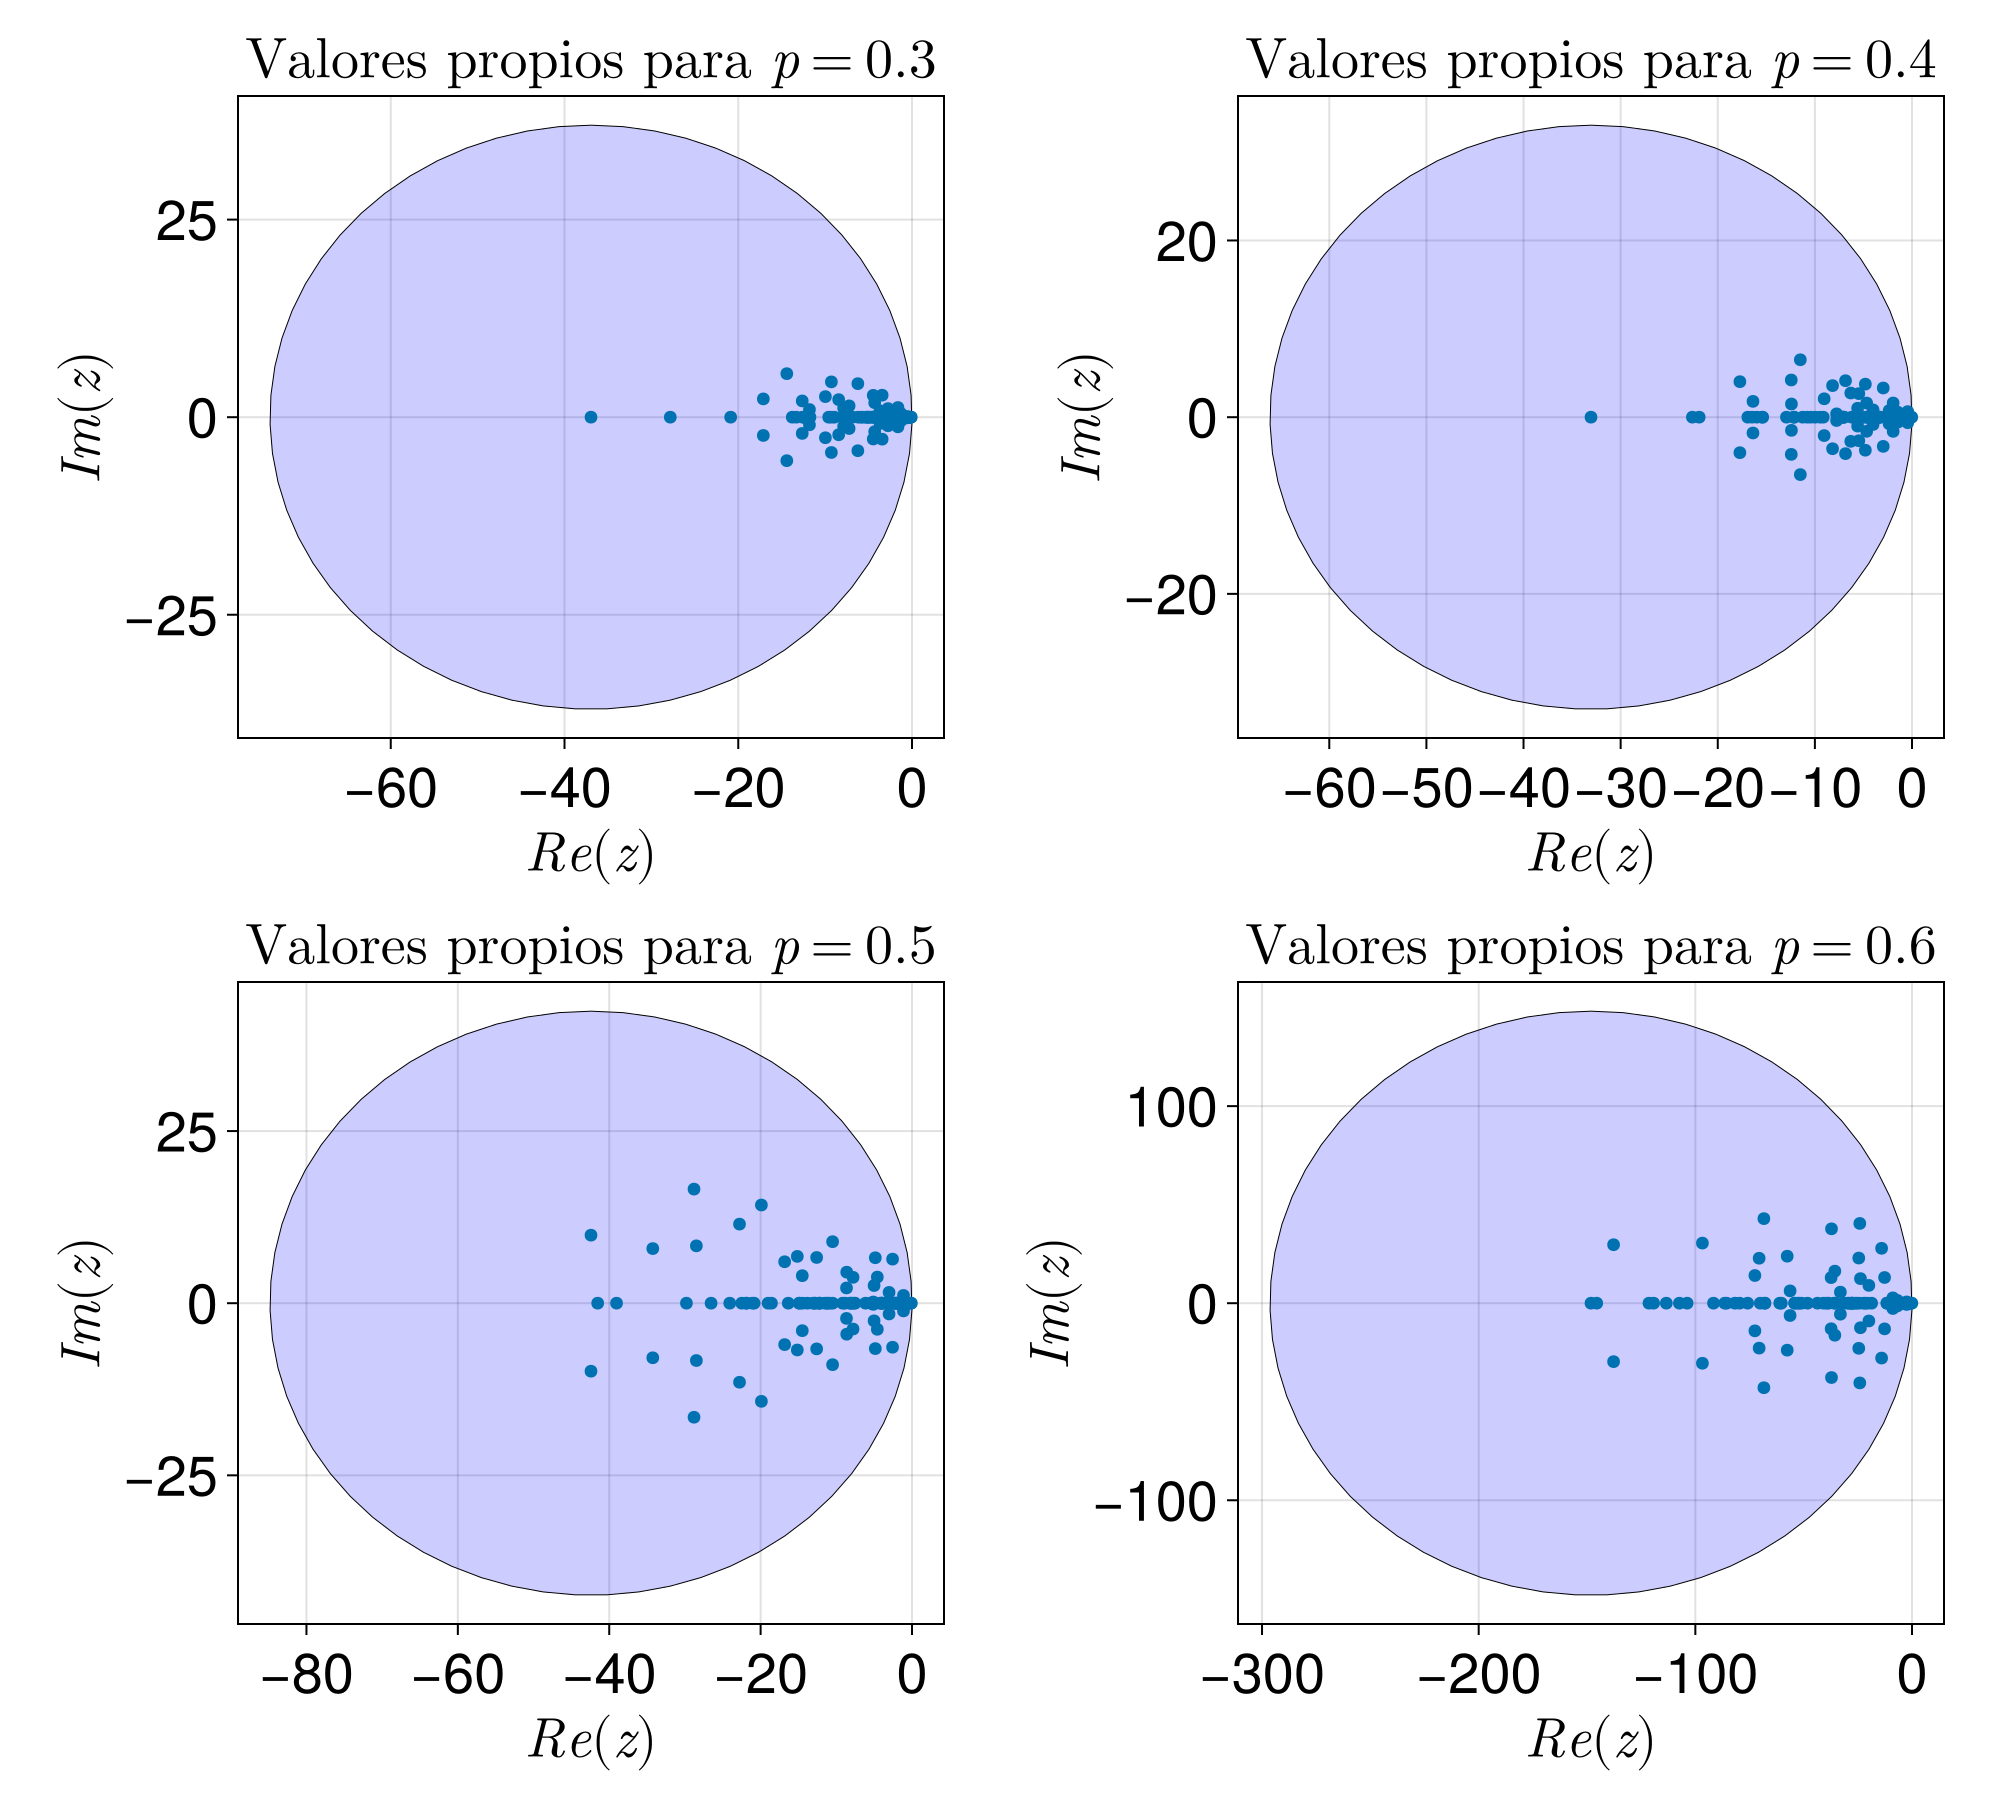
\includegraphics[scale=0.24]{../Imagenes/DistEigenvalores}
	\caption{Distribución de eigenvalores para el conjunto de jacobianos con los parámetros $N=100$, $\sigma=0.2$ y $p\in\{0.3,0.4,0.5,0.6\}$.}
	\label{fig:DistEigenvalores}
\end{figure}

Para comenzar, se ha propuesto el centro/radio como el eigenvalor con parte real mínima de cada distribución\footnote{En consecuencia se genera el Círculo con el radio más grande posible de cada sistema.}, y en primera instancia se puede observar que dicho círculo si encierra a toda la distribución de eigenvalores, además también se puede notar que en cada caso los eigenvalores cuentan con parte real negativa lo que sustenta que cada sistema sea estable. Sin embargo es notorio que la distribución no se ajusta al círculo resultante sino solamente a una parte del mismo. Otro aspecto que se puede apreciar de esta distribución es que cuanto mayor es la probabilidad de conexión entre nodos, la distribución se ensancha al igual que como ocurrió en la distribución de la diagonal Figura (\ref{fig:DistDiagonal}). \\
\\
El hecho de que la distribución de la diagonal no sea homogénea impacta directamente en la distribución de los eigenvalores, pero ¿qué pasa si en lugar de proponer una sola Ley Circular, se proponen $N$? Para ello se ocupará la distribución más ancha, con $p=0.6$ y se considerará cada valor de la diagonal de su matriz de interacciones $\mathcal{I}$ como centro y radio de una Ley Circular particular
\begin{figure}[h!]
	\centering
	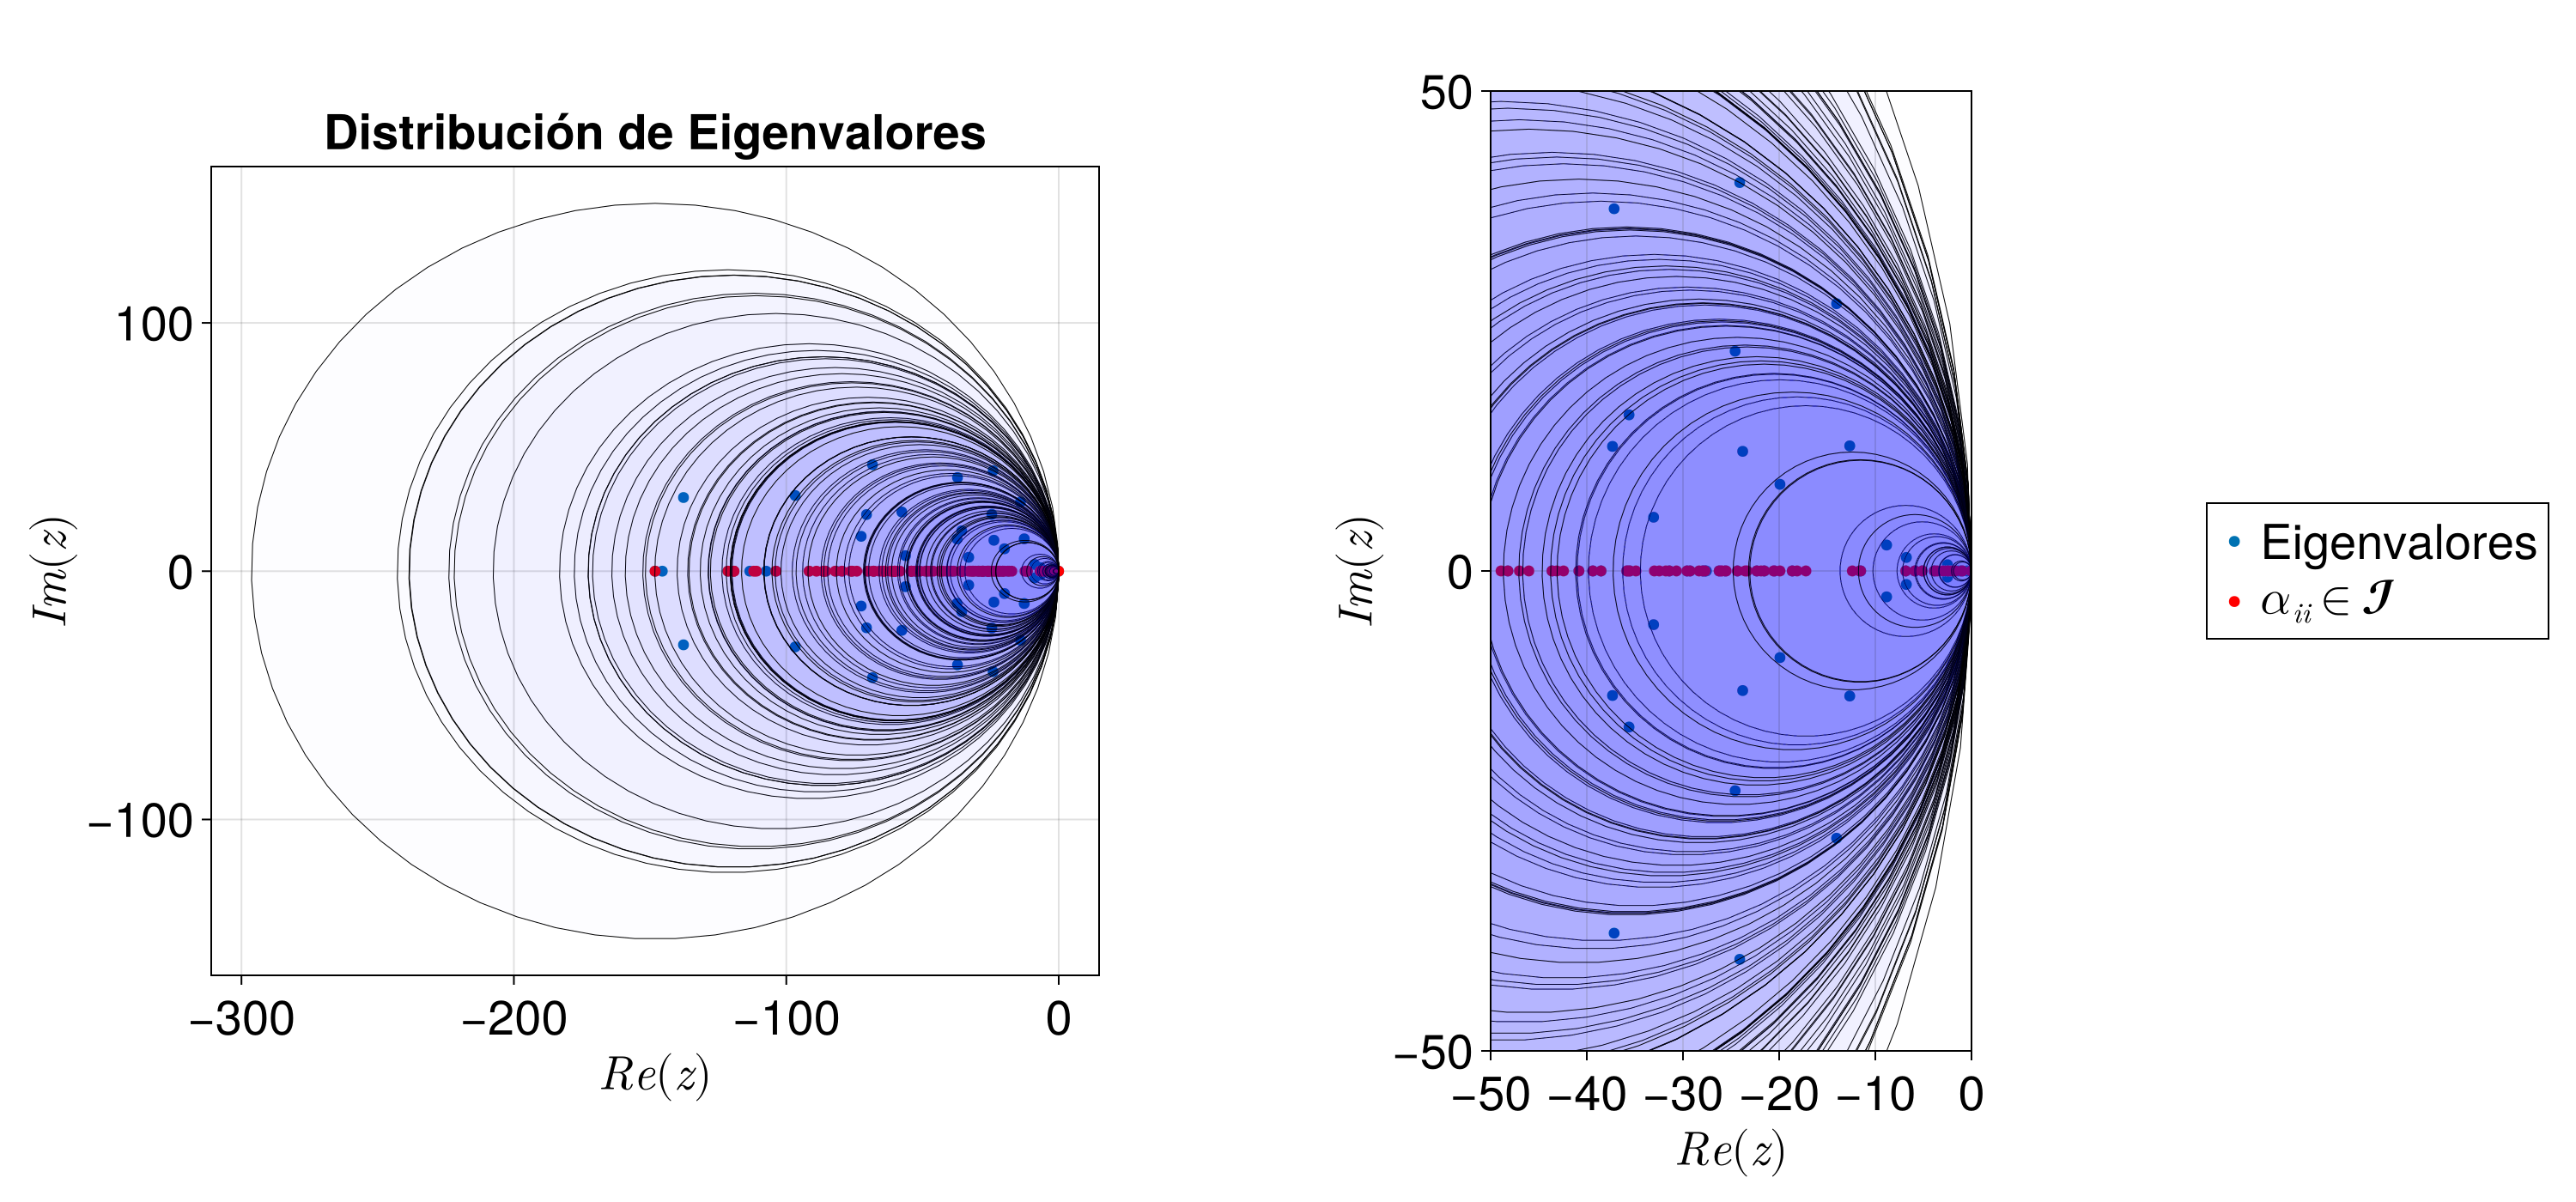
\includegraphics[scale=0.17]{../Imagenes/LeyesCirculares}
	\caption{Distribución de eigenvalores del sistema generalizado para $N=100$, $\sigma=0.2$ y $p=0.6$. Se consideran $N$ Leyes Circulares cuyo radio y centro es cada valor de la diagonal de la matriz de interacciones $\mathcal{I}$ asociada. }
	\label{fig:LeyesCirculares}
\end{figure}

Esta propuesta sugiere que cada valor de la diagonal funge como un centro y radio de una Ley Circular local que encierra cierta cantidad de eigenvalores mismos que se ajustan a dicho círculo particular. Hemos visto el mínimo valor de la distribución de la diagonal genera un Círculo que encierra 
\begin{wrapfigure}{l}{0.5 \textwidth} \vspace{-30pt} \begin{center}
	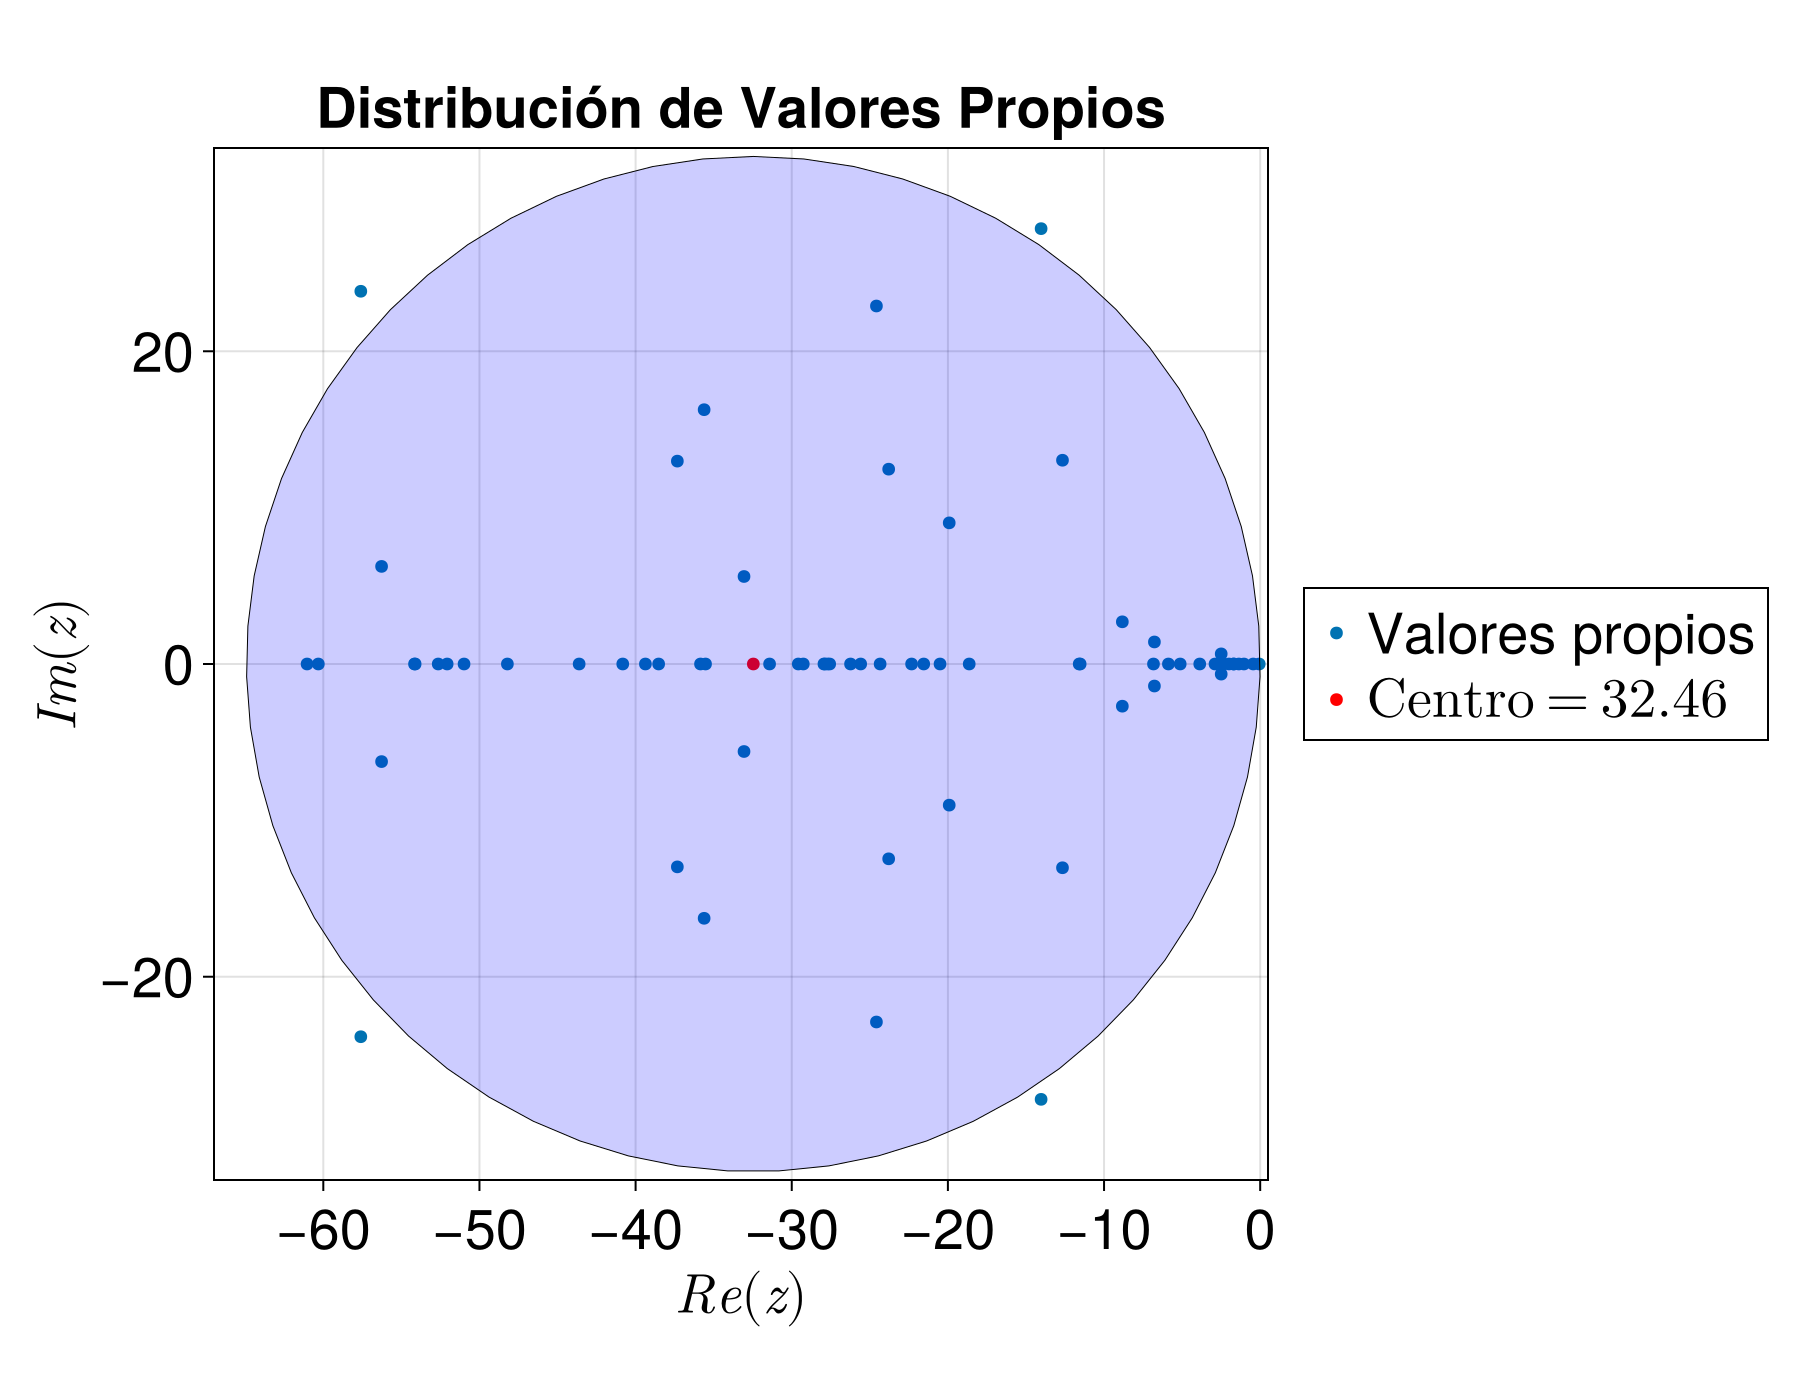
\includegraphics[scale=0.13]{../Imagenes/LeyCircularParticular}
	\end{center}
	\vspace{-20pt} 
	\caption{Caso particular de la Figura (\ref{fig:LeyesCirculares}) para el valor de la diagonal $\alpha_{ii}=32.46\in\mathcal{I}$.}
		\vspace{-50pt}
	\label{fig:LeyCircularParticular}
\end{wrapfigure}
a todos los eigenvalores pero no necesariamente la distribución se ajusta a este círculo más grande. En resumen, la propuesta que aquí se genera es que la distribución de eigenvalores de un sistema generalizado se ajusta a $N$ Leyes Circulares, mismas que se generan a partir de los valores de la diagonal de $\mathcal{I}$. De la Figura (\ref{fig:LeyesCirculares}) analicemos más de cerca un caso particular para el valor de la diagonal $\alpha_{ii}=32.46$ (Figura \ref{fig:LeyCircularParticular}), gran parte de los eigenvalores no tienen parte imaginaria sino solo la parte real negativa mientras que el resto se distribuye por el resto del círculo a excepción de algunos otros eigenvalores que pasan al siguiente nivel o siguiente círculo. Para poder confirmar o refutar esta propuesta, se necesitan de más eigenvalores dibujados en el plano complejo, ya que los eigenvalores de un solo sistema nos brinda información limitada.

\subsection{Análisis para $N=50$}

Como parte de la investigación, se tienen  a disposición un banco de \href{https://github.com/rogve98/Tesis/tree/master/Notebooks/Datos/Jacobianos}{Jacobianos} y otro de \href{https://github.com/rogve98/Tesis/tree/master/Notebooks/Datos/Diagonales}{Diagonales}\footnote{Para los Jacobianos acceder a: \url{https://github.com/rogve98/Tesis/tree/master/Notebooks/Datos/Jacobianos}. Para las Diagonales acceder a \url{https://github.com/rogve98/Tesis/tree/master/Notebooks/Datos/Diagonales}.} de Jacobianos en donde se concentran 78 archivos .csv en cada banco, y contienen cada uno la información de 100 simulaciones diferentes que resultaron ser estables. Debido al costo computacional, se tuvieron que generar para $N=50$ para los siguientes casos:
\begin{table}[h!]
	\centering
	 \begin{tabular}{|c|c|c|c|}
		\hline
		Valor promedio [$\sigma$] & Probabilidades [$p$] & Cantidad de archivos & Simulaciones realizadas \\ \hline
		$0.1-0.5$  & $0.1-1.0$  & 50 & 5000  \\ \hline
		0.6  & $0.1-0.9$  & 9 & 900 \\ \hline
		0.7  & $0.1-0.7$  & 7 & 700 \\ \hline
		0.8  & $0.1-0.5$  & 5 & 500 \\ \hline
		0.9  & $0.1-0.4$  & 4 & 400 \\ \hline
		1.0  & $0.1-0.3$  & 3 & 300 \\ \hline
		& \textbf{Total:} & 78& 7800\\ \hline
	\end{tabular}
	\caption{Cantidad de archivos generados para el banco de Diagonales y Jacobianos considerando $N=50$. A partir de $\sigma=0.6$ en adelante, los tiempos de compilación fueron muy prolongados por lo que no se obtuvieron los 10 archivos respectivos a diferencia de los valores promedio anteriores.}
	\label{tab:ejemplo}
\end{table} 

La razón de explorar sistemas estables para valores de $\sigma$ y $p$ cercanos a 1.0 era para ver que tan probable era que fueran estables en estas condiciones. Con estos datos es posible analizar como son las distribuciones de las diagonales en los sistemas que resultaron estables y por sobre todo como cambian cuando se consideran polos opuestos de $\sigma$ y $p$. Una vez viendo la distribución de las diagonales se explorará la distribución de los eigenvalores en función de los diversos $\sigma$ y $p$.

\subsubsection*{Diagonales}

Algo que se ha visualizado en un primer acercamiento (Figura (\ref{fig:DistDiagonal})) es que cuando es más grande la conectividad del sistema (parámetro $p$), la distribución de la diagonal es más amplia. Se confirmará esto con los datos disponibles y además se verá si ocurre algo similar para cuando la fuerza de interacción promedio es alta. A continuación se verán distribuciones de 5000 diagonales que fueron parte de 100 Jacobianos con $N=50$



